\documentclass[aps,pre,twocolumn,groupedaddress,amsmath,amssymb,nofootinbib]{revtex4-2}

\usepackage{bm}
\usepackage{booktabs}
\usepackage{graphicx}
\usepackage[colorlinks=true,citecolor=blue!60!black,linkcolor=blue!60!black,urlcolor=blue!60!black]{hyperref}
\usepackage{xcolor}

\newcommand{\ket}[1]{\lvert #1\rangle}
\newcommand{\bra}[1]{\langle #1\rvert}
\newcommand{\proj}[1]{\ket{#1}\!\bra{#1}}
\newcommand{\Tr}{\operatorname{Tr}}
\newcommand{\W}{\mathcal{W}}

\begin{document}

\title{Collisional harvesting of renewed coherence:
impedance matching and accessible ergotropy}

\author{Noufal Jaseem}
\affiliation{Department of Physical Sciences, Indian Institute of Science Education and Research Berhampur, India}
\author{Bitan De}
\affiliation{Institute of Theoretical Physics, Jagiellonian University in Krak\'{o}w, Lojasiewicza 11, 30-348 Krak\'{o}w, Poland}
\author{Parvinder Solanki}
\affiliation{Department of Physics, Indian Institute of Technology Bombay, Powai, Mumbai 400076, India}
\author{Sai Vinjanampathy}
\email{sai@phy.iitb.ac.in}
\affiliation{Department of Physics, Indian Institute of Technology Bombay, Powai, Mumbai 400076, India}
\affiliation{Centre for Quantum Technologies, National University of Singapore, 3 Science Drive 2, 117543 Singapore, Singapore}
\author{Bhaskaran Muralidharan}
\email{bm@ee.iitb.ac.in}
\affiliation{Department of Electrical Engineering, Indian Institute of Technology Bombay, Powai, Mumbai 400076, India}
\date{\today}

\begin{abstract}
We study continuous conversion of a renewed quantum coherence into the
ergotropy of a tape of qubit batteries. A V-type three-level system carries
coherence in a split excited doublet and collides, one by one, with
ground-state ancillas through a resonant exchange that conserves bare energy
and the intended excitation number. We derive the exact collision map, the
stroboscopic fixed point under a renewal bath, and the outgoing qubit
ergotropy. The main question is simple: what collision rate maximizes the
charging power? We show that the optimum is an impedance match between
coherence regrowth and collisional depletion. In the weak-collision limit
this gives a broad plateau and a closed law for finite precession of the
gap. We also separate total ergotropy from work that can be accessed without
a phase reference, and we give the full three-regime result for two
energy-dephased copies. The model is a companion theory for coherence
harvesting. It is not a claim about restoring electrical transport power.
\end{abstract}

\maketitle

\section{Introduction}

Quantum coherence can change the work that can be drawn from a finite
system. Ergotropy and work that can actually be extracted coincide only
after the allowed operations and the available reference resources are
fixed~\cite{Allahverdyan2004,Francica2020,Lostaglio2015}. Quantum batteries
make this distinction concrete: one cares not only how much energy is
stored, but how fast a useful nonpassive state can be
prepared~\cite{AlickiFannes2013,Campaioli2017}. Repeated interactions give a
natural continuous setting, in which a system collides with a stream of
fresh probes~\cite{Bettmann2023,Prositto2025,CollisionalTransmon2025,NoGo2026}.

Long-lived coherence in a V-type three-level system has recently been
studied as a work resource~\cite{Chen2025}. Our question is sharper.
\emph{If that coherence is renewed between collisions, can it charge a
battery tape continuously, and what limits the power?} In particular: is
there a simple matching condition between the rate at which the bath
rebuilds coherence and the rate at which collisions remove it?

We answer this with a minimal model. A V-type system with a coherent
excited doublet interacts with ground-state ancillas through a matched-gap
exchange. The collision itself needs no external work. We derive the exact
channel and the fixed point, find the power optimum, and quantify the
penalties from finite precession and finite coupling. We also separate total
ergotropy from work that is accessible under stated discharge rules.
Long-lived V-system coherence is the resource; the continuous, stroboscopic
conversion law and its impedance-matched power optimum are our
contribution.

We report total ergotropy as an upper bound on battery work capacity.
Without a phase reference, the coherent part of a single outgoing ancilla
is not freely extractable by energy-preserving operations alone; that
distinction is made precise in Sec.~\ref{sec:access}.

\section{Matched-gap collision model}

The system basis is $\{\ket{0},\ket{1},\ket{2}\}$. We use the doublet
variables
\begin{equation}
s=\rho_{11}+\rho_{22},\qquad d=\rho_{11}-\rho_{22},\qquad C=\rho_{12}.
\end{equation}
The free Hamiltonians are matched at a finite gap $\Delta$,
\begin{align}
H_S&=\bar E(\proj{1}+\proj{2})
 +\frac{\Delta}{2}(\proj{1}-\proj{2}),\\
H_A&=\Delta\proj{\uparrow}.
\end{align}
A fresh ancilla has excited population $\alpha$ and no coherence. During a
collision of duration $\tau$,
\begin{equation}
H_{\rm int}=\hbar g\bigl(
 \ket{1\downarrow}\bra{2\uparrow}
+\ket{2\uparrow}\bra{1\downarrow}\bigr),\qquad \theta=g\tau .
\label{eq:hint}
\end{equation}
On the active block, $H_S+H_A$ is proportional to the identity, so
$[H_S+H_A,H_{\rm int}]=0$. The same exchange conserves the intended
excitation number. A finite matched $\Delta>0$ is essential. At exact
doublet degeneracy, strict resonance would force a gapless ancilla, which
cannot store energetic ergotropy.

\begin{figure*}[t]
\includegraphics[width=\textwidth]{../figures/companion_scheme.pdf}
\caption{Renewal rebuilds the V-system doublet coherence between exchange
collisions. Independent outgoing qubits carry energy and ergotropy. The
analytic reset is phase locked. The directed-leakage bath gives an
autonomous comparison in the weak-collision regime.}
\label{fig:scheme}
\end{figure*}

Tracing the exact unitary $U_\theta=\exp(-iH_{\rm int}\tau/\hbar)$ yields
\begin{subequations}
\begin{align}
s'&=s,\\
d'&=\cos^2\theta\,d-\sin^2\theta(1-2\alpha)s,\\
C'&=\cos\theta\,C.
\end{align}
\label{eq:map}
\end{subequations}
The outgoing ancilla Bloch components are
\begin{subequations}
\begin{align}
p_\uparrow'&=\alpha+\frac{\sin^2\theta}{2}
   \bigl[s(1-2\alpha)+d\bigr],\\
\rho_{\uparrow\downarrow}'&=-i\sin\theta(1-2\alpha)C,\\
z_A&=2p_\uparrow'-1,\quad
x_A=2\Re\rho_{\uparrow\downarrow}',\quad
y_A=-2\Im\rho_{\uparrow\downarrow}' .
\end{align}
\label{eq:ancilla}
\end{subequations}
Direct $6\times6$ unitary propagation agrees with
Eqs.~(\ref{eq:map})--(\ref{eq:ancilla}) to floating-point precision
(Fig.~\ref{fig:validation}).

\section{Renewal and stroboscopic coherence}

We use two renewal pictures. The analytic benchmark is an affine,
phase-locked reset over the waiting time $T=1/r$:
\begin{align}
C_{n+1}&=q_C e^{-i\phi}\cos\theta\,C_n+(1-q_C)c_0,\nonumber\\
q_C&=e^{-\gamma_C/r},\qquad \phi=\Delta/r .
\end{align}
Its fixed point is exact:
\begin{equation}
C^*=\frac{(1-q_C)c_0}
 {1-q_C e^{-i\phi}\cos\theta}.
\label{eq:cstar}
\end{equation}
Population relaxation is treated by a separate factor
$q_d=e^{-\gamma_d/r}$ and is kept in the numerical curves.

A lab-frame steady coherence at finite splitting is not automatic for a
single undriven thermal bath. The affine map must be justified. We do this
with a directed dark-state-leakage bath: bright-state pumping and relaxation
$(\Gamma_\uparrow,\Gamma_\downarrow)$ plus dark leakage at rate $\kappa_D$,
\begin{equation}
\dot p_B=\Gamma_\uparrow p_0-\Gamma_\downarrow p_B,\qquad
\dot p_D=-\kappa_D p_D,\qquad p_0=1-p_B-p_D.
\label{eq:leakage}
\end{equation}
Its steady state is $p_D^{\rm ss}=0$ and
$p_B^{\rm ss}=\Gamma_\uparrow/(\Gamma_\uparrow+\Gamma_\downarrow)\equiv
s_{\rm ss}$. The real doublet coherence is the bright--dark imbalance,
$C=(p_B-p_D)/2$, so the bath stabilizes
\begin{equation}
c_0=\frac{s_{\rm ss}}{2}
\end{equation}
by itself. When the rates match,
$\kappa_D=\Gamma_\uparrow+\Gamma_\downarrow\equiv\gamma_C$, the waiting-time
map of Eq.~(\ref{eq:leakage}) reduces to the affine reset with
$q_C=e^{-\gamma_C/r}$ and $c_0=s_{\rm ss}/2$, up to $O(\theta^2)$
corrections from the dark population made by the collision
(Appendix~\ref{app:leakage}). The power optimum sits in this weak-collision
regime, so the main formulas
[Eqs.~(\ref{eq:cstar}) and (\ref{eq:optimum})] use microscopically fixed
$\gamma_C$ and $c_0$. Away from matched rates we keep the full
two-dimensional affine map and solve it numerically
(Fig.~\ref{fig:robust-access}). The phase $e^{-i\phi}$ is free precession at
the finite gap. The fully autonomous, phase-unreferenced reading of our
results is safest for $\delta=\Delta/\gamma_C\lesssim 1$, where
Eq.~(\ref{eq:optimum}) already gives the precession penalty. Symmetric
bright--dark mixing is \emph{not} a renewal mechanism: it equalizes the two
populations and kills $C$.

\begin{figure*}[t]
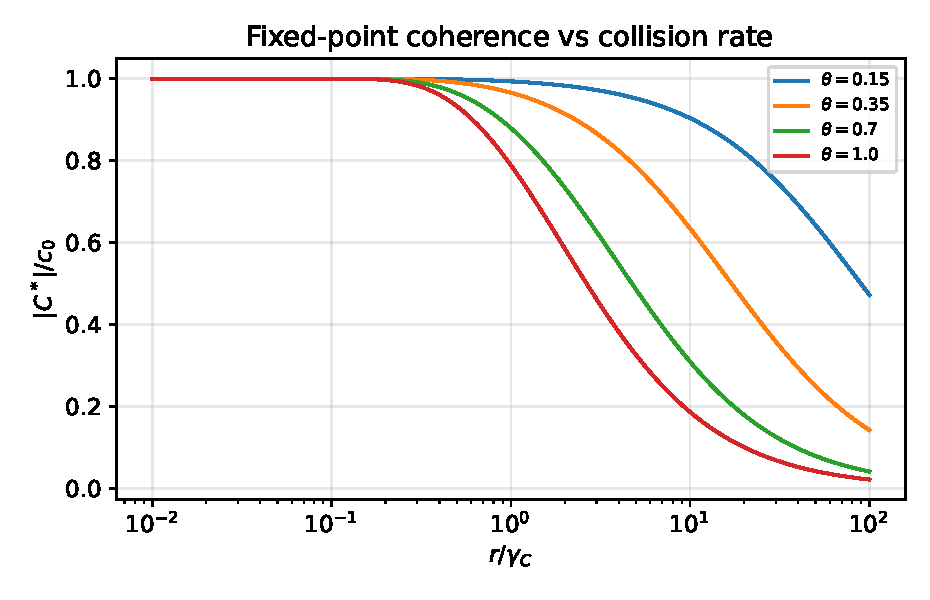
\includegraphics[width=.49\textwidth]{../figures/companion_Cstar_vs_r.pdf}
\hfill
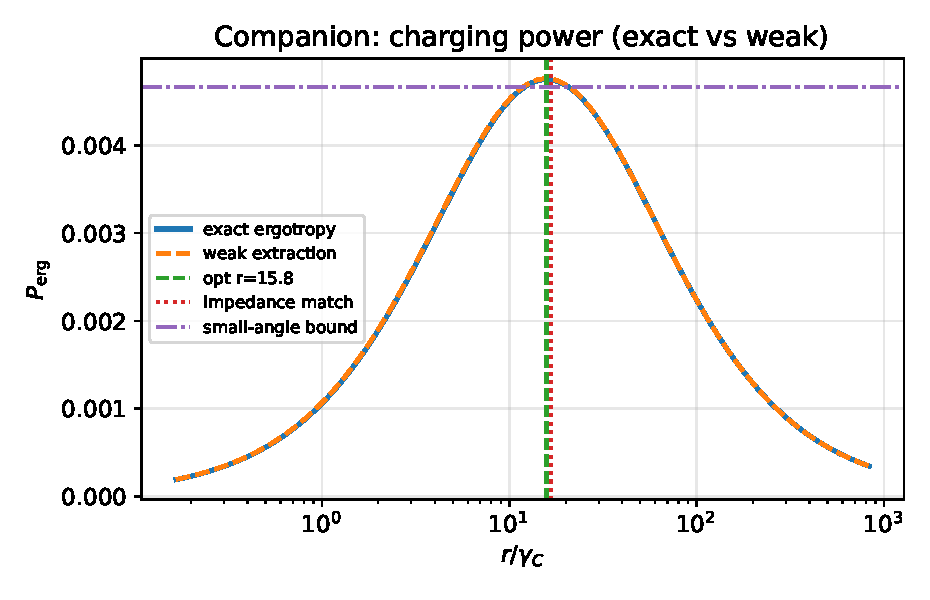
\includegraphics[width=.49\textwidth]{../figures/companion_power_curve.pdf}
\caption{Left: fixed-point coherence under renewal and collisional depletion
at zero precession. Right: exact power and weak-extraction approximation for
$(\gamma_C,\gamma_d,c_0,s_{\rm ss},\Delta,\theta,\alpha)
=(1,1,0.25,0.5,0.15,0.35,0)$.}
\label{fig:fixed-power}
\end{figure*}

\section{Ergotropy and impedance matching}

For a qubit with Hamiltonian $H_A=\Delta\proj{\uparrow}$, Bloch length
$|\bm r_A|$, and vertical component $z_A$, the ergotropy is
\begin{equation}
\W_A=\frac{\Delta}{2}\bigl(z_A+|\bm r_A|\bigr).
\label{eq:ergotropy}
\end{equation}
In the weak-extraction, ground-biased regime,
\begin{equation}
\W_A\simeq
\frac{\Delta\sin^2\theta\,|C^*|^2}{|z_A|},
\qquad P_{\rm erg}=r\W_A.
\label{eq:weak}
\end{equation}
Define the extraction rate
\begin{equation}
\Gamma_{\rm ext}=r(1-\cos\theta).
\end{equation}
At small precession, maximizing Eq.~(\ref{eq:weak}) gives a simple answer:
\begin{equation}
\Gamma_{\rm ext}\simeq\gamma_C.
\end{equation}
Extraction faster than renewal depletes $C^*$. Extraction slower than
renewal wastes regenerated coherence. That is the impedance match. For
$\delta=\Delta/\gamma_C$, the small-angle optimum and bound become
\begin{subequations}
\begin{align}
r_{\rm opt}&\simeq
 \frac{\gamma_C\sqrt{1+\delta^2}}{1-\cos\theta},\\
P_{\rm erg}^{\max}(\delta)&\simeq
 \frac{\gamma_C\Delta c_0^2}{|z_A|}
 \frac{1}{1+\sqrt{1+\delta^2}}.
\end{align}
\label{eq:optimum}
\end{subequations}
So $P_{\max}(0)=\gamma_C\Delta c_0^2/(2|z_A|)$, and the normalized
finite-phase suppression is $2/[1+\sqrt{1+\delta^2}]$.

\begin{figure*}[t]
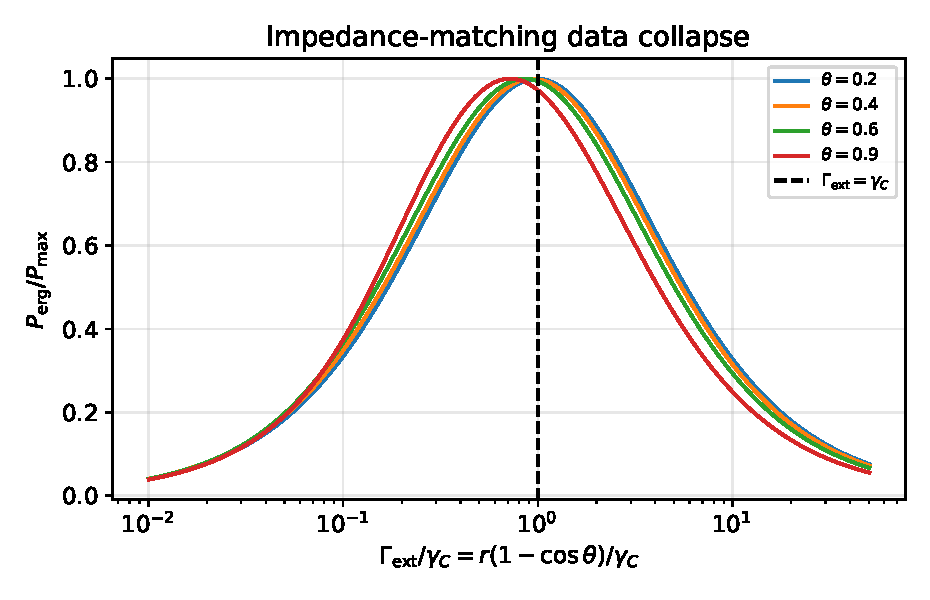
\includegraphics[width=.49\textwidth]{../figures/companion_impedance_collapse.pdf}
\hfill
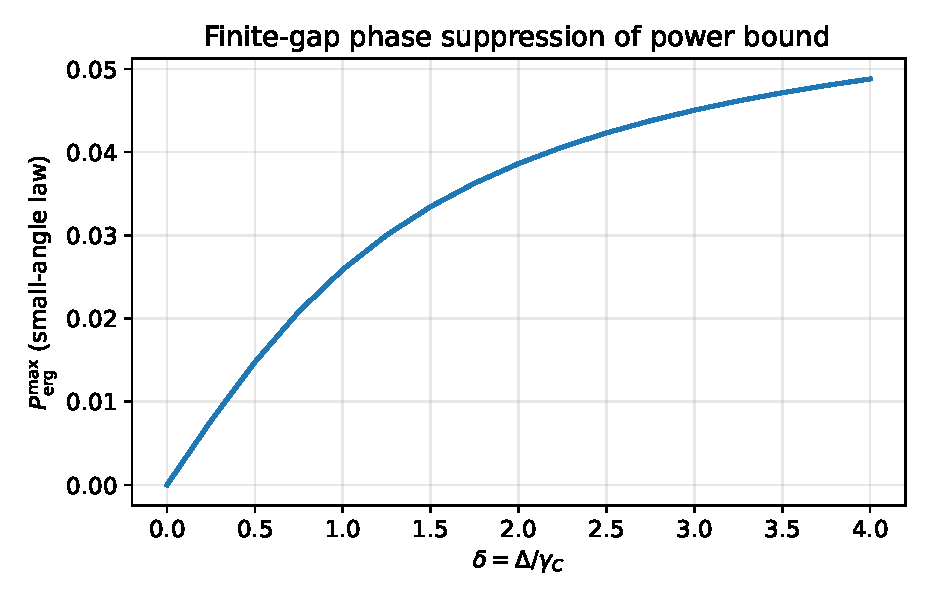
\includegraphics[width=.49\textwidth]{../figures/companion_finite_phase_bound.pdf}
\caption{Left: normalized exact power collapses around
$\Gamma_{\rm ext}/\gamma_C=1$. Right: finite-precession suppression with
the energy prefactor held fixed, so the plot isolates phase detuning from
the linear factor of $\Delta$ in the ergotropy.}
\label{fig:impedance}
\end{figure*}

At zero phase the finite-angle harvesting prefactor is almost flat,
\begin{equation}
\mathcal C(\theta)=\frac12-\frac{\theta^4}{96}+O(\theta^6).
\end{equation}
The formal limit $\theta\to0$, $r\to\infty$ is not free: $\theta=g\tau\le g/r$.
At the optimum this requires
\begin{equation}
\theta\gtrsim
\frac{2\gamma_C\sqrt{1+\delta^2}}{g}.
\label{eq:realizability}
\end{equation}
The bound is linear, not square-root, in $\gamma_C/g$.

\section{Accessible work}
\label{sec:access}

Equation~(\ref{eq:ergotropy}) is the maximum under unrestricted unitaries.
Without a phase reference, time-translation-covariant one-copy discharge
first dephases between distinct energies. What remains is
\begin{equation}
\W_{\rm acc}^{(1)}=\W_{\rm inc}.
\end{equation}
For the purely coherent, ground-biased outputs we study, this is zero. An
explicit phase reference can unlock the total ergotropy, but then the
reference itself is part of the resource budget~\cite{Lostaglio2015}.

Two copies keep relational coherence inside the one-excitation sector. Write
one output as
\begin{equation}
\rho_A=\begin{pmatrix}a&c\\c^*&b\end{pmatrix},
\qquad a+b=1,\quad a\ge b .
\end{equation}
After total-energy dephasing of $\rho_A^{\otimes2}$, eigenvalue sorting gives
\begin{equation}
\W_{\rm acc}^{(2)}=
\begin{cases}
0,& |c|^2\le b(a-b),\\
\Delta[|c|^2-b(a-b)],
 & b(a-b)<|c|^2\le a(a-b),\\
\Delta[2|c|^2-(a-b)],
 & a(a-b)<|c|^2\le ab.
\end{cases}
\label{eq:twocopy}
\end{equation}
The weak-harvesting curves usually stay below the first threshold. We
therefore report total ergotropy as an upper bound, not as work that is
automatically available from one or two batteries.

\begin{figure*}[t]
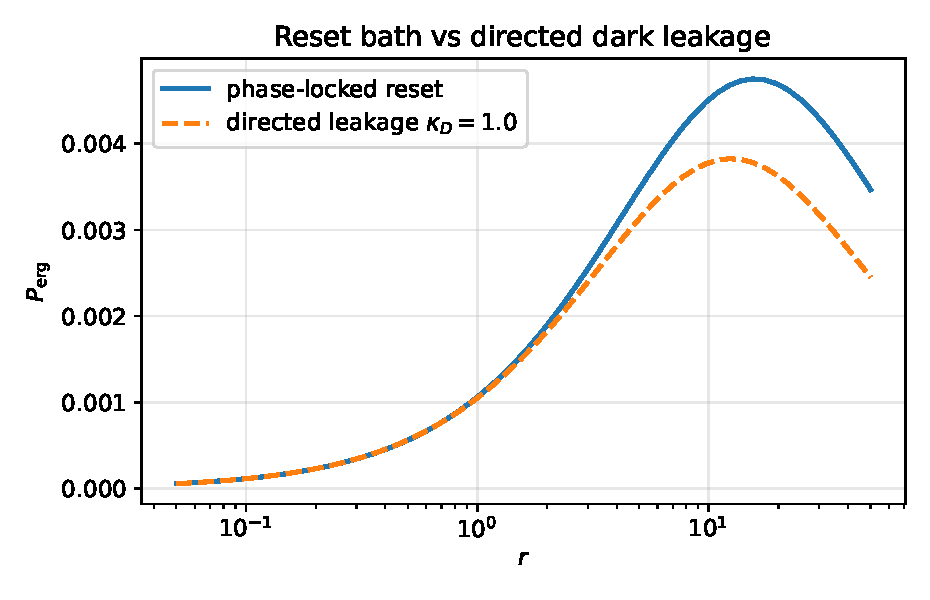
\includegraphics[width=.49\textwidth]{../figures/companion_reset_vs_leakage.pdf}
\hfill
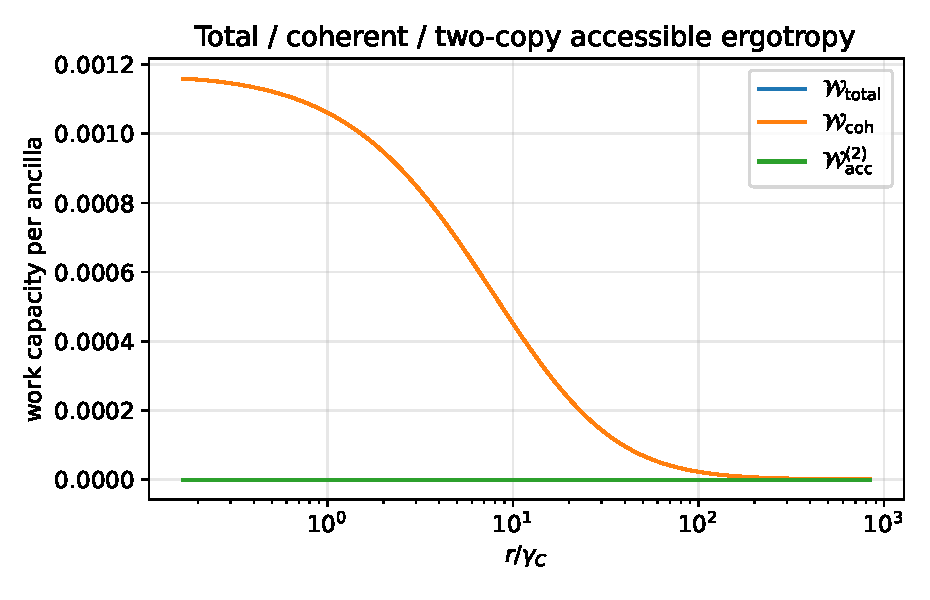
\includegraphics[width=.49\textwidth]{../figures/companion_accessibility.pdf}
\caption{Left: phase-locked reset versus directed dark leakage, including
the retained coherence and the minimum physicality margin over the scanned
rates. Right: total and coherent ergotropy compared with one- and two-copy
work after the stated energy dephasings.}
\label{fig:robust-access}
\end{figure*}

\section{Discussion}

The model shows a simple rate-matching rule: the gross charging power is
largest when collisional depletion and coherence regrowth are comparable.
Finite-angle numerics keep this picture. Precession only multiplies the
bound by a closed dimensionless factor. In the weak-collision window where
the optimum sits, the affine map, $\gamma_C$, and $c_0$ all follow from the
directed dark-state-leakage bath
(Appendix~\ref{app:leakage}). Away from matched rates the power degrades, as
shown by the leakage scan, and physicality checks keep unphysical coherence
out of the comparison.

Some costs sit outside the gross power in Eq.~(\ref{eq:optimum}).
Ground-state ancillas are low-entropy resources; their preparation free
energy must enter any net efficiency. A phase reference used at discharge is
likewise a resource. These points do not change the collision map or the
impedance match. They do limit the thermodynamic claim.

A transport-driven spin valve can regenerate coherence and also produce
electrical power. That extension needs a lead-resolved nonsecular generator,
positivity checks, and a real electrical-power/ergotropy tradeoff. It is not
part of the present companion result.

\section{Conclusion}

A resonant, charge-preserving exchange converts renewed V-system coherence
into a stream of nonpassive qubit states. The stroboscopic solution gives
impedance matching, a flat finite-angle plateau, and a finite-precession
penalty. The operational statement is narrower than the gross ergotropy
alone: without a phase reference the one-copy coherent part is locked, and
two-copy activation follows the thresholds in Eq.~(\ref{eq:twocopy}). These
distinctions put the coherence-harvesting bound on a clear thermodynamic
footing.

\begin{acknowledgments}
The idea of coupling an ancilla tape to a coherence-generating open system,
in order to harvest coherence as battery ergotropy, was conceived by S.V.\
and B.M. N.J.\ developed the companion model and the analytic and numerical
results. All authors contributed to checking and improving the results and
the manuscript.
\end{acknowledgments}

\appendix

\section{Unitary channel check}

In the ordered active basis
$\{\ket{1\downarrow},\ket{2\uparrow}\}$,
\begin{equation}
U_\theta=
\begin{pmatrix}
\cos\theta&-i\sin\theta\\
-i\sin\theta&\cos\theta
\end{pmatrix}.
\end{equation}
Embedding this block in the six-dimensional product space and tracing the
ancilla reproduces Eq.~(\ref{eq:map}). The validation samples physical
doublet states and random $\theta,\alpha$; the error data are exported with
the figures.

\section{Reduction of directed leakage to the affine renewal}
\label{app:leakage}

With $A=\Gamma_\uparrow+\Gamma_\downarrow$, $q_B=e^{-A\tau_c}$,
$q_D=e^{-\kappa_D\tau_c}$, the waiting-time map of Eq.~(\ref{eq:leakage})
from post-collision values $(B_+,D_+)$ is
\begin{equation}
D_-=q_D D_+,\qquad
B_-=q_B B_+ + s_{\rm ss}(1-q_B)
-\Gamma_\uparrow D_+\frac{q_D-q_B}{A-\kappa_D},
\end{equation}
while the collision acts as
$(B_+,D_+)^T=R_\theta(B_-,D_-)^T$ with
$R_\theta=\tfrac12\bigl(\begin{smallmatrix}
1+\cos\theta&1-\cos\theta\\ 1-\cos\theta&1+\cos\theta
\end{smallmatrix}\bigr)$.
At matched rates $\kappa_D=A\equiv\gamma_C$ one has $q_B=q_D=q_C$ and the
cross term becomes $\Gamma_\uparrow D_+\tau_c e^{-\gamma_C\tau_c}$. The
collision generates dark population only at second order,
$D_+=\tfrac{1-\cos\theta}{2}(B_--D_-)=O(\theta^2)$, so to leading order in
$\theta$ the imbalance $C=(B-D)/2$ obeys
\begin{equation}
C_{n+1}=q_C\cos\theta\,C_n+(1-q_C)\,\frac{s_{\rm ss}}{2},
\end{equation}
which is the affine benchmark with $\gamma_C=\kappa_D=A$ and
$c_0=s_{\rm ss}/2$. Because the power optimum obeys
$1-\cos\theta\simeq\gamma_C/r\ll1$, the neglected terms enter the fixed point
at relative order $\theta^2$ and the optimal power at order $\theta^4$, in
line with the flat plateau. The mismatched-rate case is the two-dimensional
affine map used for Fig.~\ref{fig:robust-access}.

\section{Two-copy eigenvalue ordering}

Total-energy dephasing leaves populations $a^2$ and $b^2$ at energies
$0$ and $2\Delta$, and a one-excitation block
\begin{equation}
\begin{pmatrix}ab&|c|^2\\|c|^2&ab\end{pmatrix}
\end{equation}
with eigenvalues $ab\pm|c|^2$. Pairing decreasing eigenvalues with the
energy list $\{0,\Delta,\Delta,2\Delta\}$ yields Eq.~(\ref{eq:twocopy}).
The boundaries are $ab-|c|^2=b^2$ and $ab+|c|^2=a^2$. Positivity enforces
$|c|^2\le ab$.

\begin{figure*}[t]
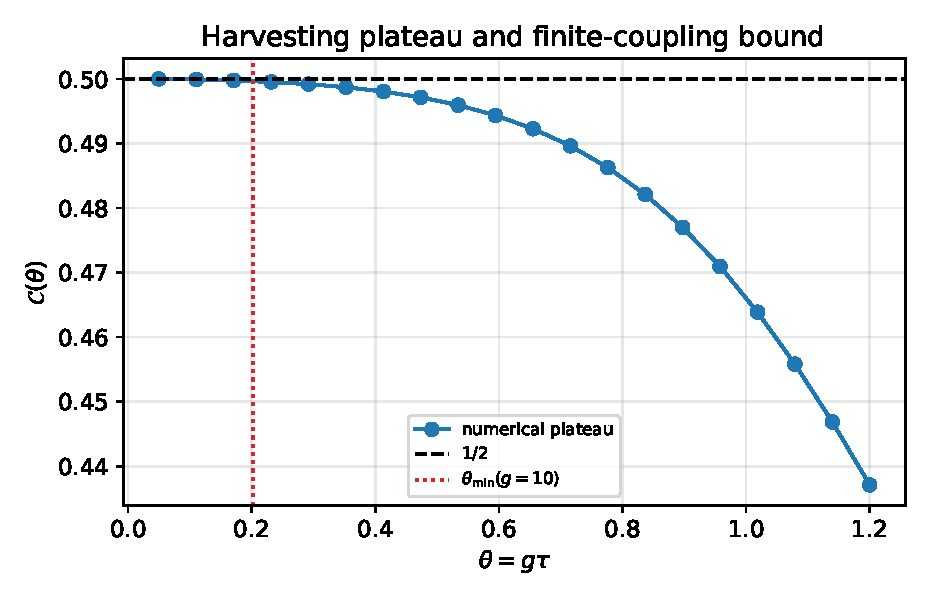
\includegraphics[width=.32\textwidth]{../figures/companion_plateau.pdf}
\hfill
\includegraphics[width=.32\textwidth]{../figures/companion_weak_approximation_error.pdf}
\hfill
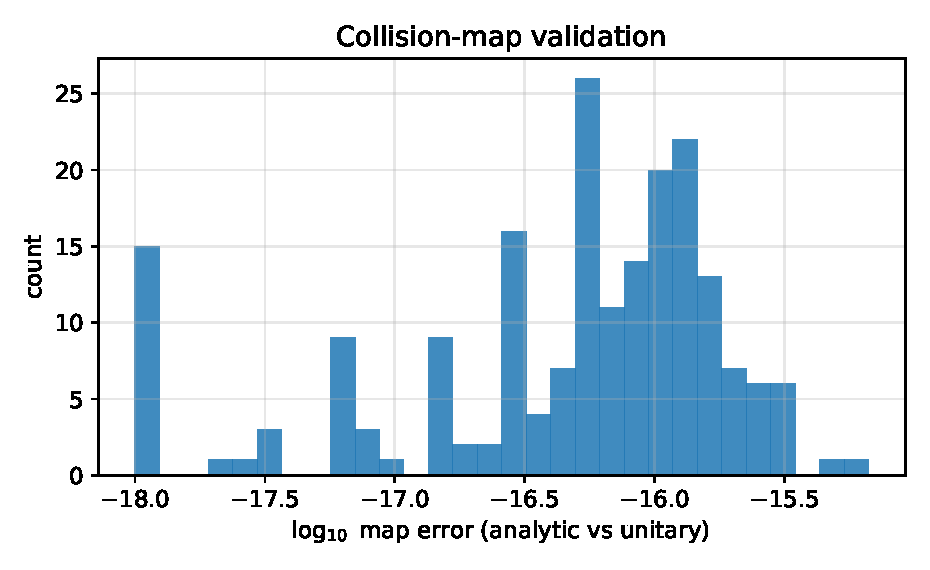
\includegraphics[width=.32\textwidth]{../figures/companion_collision_validation.pdf}
\caption{Checks beyond the main power curves. Left: finite-angle plateau and
realizability threshold. Center: accuracy of the weak-extraction formula.
Right: analytic-channel error against direct unitary propagation for random
physical input states.}
\label{fig:validation}
\end{figure*}

\bibliography{references}

\end{document}
